\chapter{General Terminology}
\begin{idea}
\begin{itemize}
  \item Introduction to AI terminology and approaches: \textbf{symbolic} and \textbf{connectionist}.
  \item \textbf{Symbolic Approach}: Logic-based problem-solving with strengths in transparency and reasoning, but struggles with complexity and contextual understanding.
  \item \textbf{Connectionist Approach (Neural Networks)}: Brain-inspired networks for pattern recognition with adaptability, but challenges in interpretability and overfitting.
  \item AI covers fields like \textbf{ML}, \textbf{CV}, \textbf{NLP}.
  \item Machine learning \textbf{learns from data} without explicit programming.
  \item Deep learning (DL) is a \textbf{subset of ML with multi-level abstractions}.
  \item DL \textbf{excels} in translation, image generation, gaming; faces \textbf{challenges} in interpretability and bias.
  \item Learning categories: \textbf{supervised}, \textbf{unsupervised}, \textbf{reinforcement}.
  \item \textbf{Bias-Variance Tradeoff} balances model complexity for better generalization.
  \item Splitting datasets for \textbf{training, validation, testing} aids model performance and selection.
\end{itemize}
\end{idea}
\section{Artificial Intelligence}
\begin{itemize}
    \item AI was coined in 1956 with the hope to \textbf{reproduce human intelligence} with machines.
    \item It captures the notion of developing computer systems that can perform tasks normally only humans can.
    \item AI is a \textbf{poorly defined} term and its meaning has changed with time
    \item Historically, there have been two distinct approaches to AI: 
\end{itemize}

\begin{enumerate}
    \item \textbf{Symbolic Approach}
    \begin{definition}
    The \textbf{symbolic} approach to AI is based on the idea that intelligent behavior can be achieved by \textbf{manipulating symbols or abstract representations of concepts and their relationships}. It draws inspiration from \textbf{formal logic} and relies on \textbf{rules, logic, and symbolic representation of knowledge} to solve problems. In this approach, knowledge is typically represented using symbols, such as predicates, rules, and frames, and reasoning involves manipulating these symbols using logical inference.
\end{definition}
\begin{figure}[h!t]
    \centering
    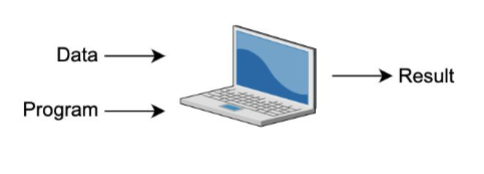
\includegraphics[width=0.5\linewidth]{symbolic.png}
    \caption{Symbolic Approach}
    \label{fig:enter-label}
\end{figure}
\begin{enumerate}
    \item \textbf{Key Characteristics}:
    \begin{enumerate}
        \item \textbf{"Model the knowledge of an adult"}
        \item \textbf{Symbol Manipulation}: The approach focuses on manipulating symbols according to predefined rules and logic.
        \item \textbf{Knowledge Representation}: Information is represented using explicit symbols, which can represent concepts, relationships, and facts.
        \item \textbf{Rule-Based Systems}: AI systems in this approach often use rule-based systems to infer conclusions from given premises.
        \item \textbf{Logic and Inference}: Logical reasoning is a core component of this approach, and it's used to derive new information from existing knowledge.
        \item \textbf{Expert Systems}: Early AI applications like expert systems used the symbolic approach, where human expertise was encoded in the form of rules and facts.
    \end{enumerate}
    \item \textbf{Strengths}:
        \begin{enumerate}
        \item \textbf{Transparency}: Symbolic systems provide a clear and interpretable representation of knowledge and reasoning processes.
        \item \textbf{Logical Reasoning}: Well-suited for problems that require logical inference and deductive reasoning.
        \item \textbf{Human-Readable}: The representations used are often human-readable and understandable.
    \end{enumerate}
    \item \textbf{Weaknesses}:
            \begin{enumerate}
        \item \textbf{Complexity}: Symbolic approaches can struggle with managing and representing the complexity of real-world domains.
        \item \textbf{Knowledge Acquisition}: Constructing a comprehensive set of rules and knowledge for complex domains can be challenging.
        \item \textbf{Lack of Contextual Understanding}: Symbolic systems may struggle with tasks that require understanding context and handling ambiguous or incomplete information.
    \end{enumerate}
\end{enumerate}
    \item \textbf{Connectionist Approach}
\begin{definition}
The \textbf{connectionist} approach, also known as the \textbf{neural network} approach, draws inspiration from the \textbf{structure and function of the human brain}. It involves building \textbf{artificial neural networks} that consist of \textbf{interconnected nodes (neurons)} that process information in a parallel and distributed manner. These networks learn patterns and relationships from data through \textbf{training processes} that adjust the strengths of connections (weights) between neurons.
\end{definition}
\begin{figure}[h!t]
    \centering
    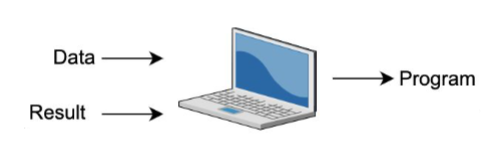
\includegraphics[width=0.5\linewidth]{connectionist.png}
    \caption{Connectionist Approach}
    
    \label{fig:enter-label}
\end{figure}
\begin{enumerate}
    \item \textbf{Key Characteristics}:
    \begin{enumerate}
        \item \textbf{"Simulate the learning of a baby"}
        \item \textbf{Parallel Distributed Processing}: Information processing occurs in parallel across interconnected nodes, leading to emergent properties.
        \item \textbf{Learning from Data}: Neural networks learn patterns and relationships from large datasets through processes like supervised learning, unsupervised learning, and reinforcement learning.
        \item \textbf{Feature Extraction}: Neural networks can automatically learn relevant features from raw data, reducing the need for hand-crafted feature engineering.
        \item \textbf{Nonlinear Mapping}: Neural networks can capture complex nonlinear relationships in data.
    \end{enumerate}
    \item \textbf{Strengths}:
        \begin{enumerate}
        \item \textbf{Pattern Recognition}: Excellent at tasks such as image recognition, natural language processing, and other tasks involving pattern recognition.
        \item \textbf{Adaptability}: Neural networks can learn from data and adapt to different tasks with appropriate training.
        \item \textbf{Robustness}: Neural networks can generalize well to new data, even in the presence of noise or variability.
    \end{enumerate}
    \item \textbf{Weaknesses}:
            \begin{enumerate}
        \item \textbf{Black Box Nature}: Neural networks can be challenging to interpret, and understanding their decision-making processes can be difficult.
        \item \textbf{Data Dependency}: Neural networks require substantial amounts of data for effective training.
        \item \textbf{Overfitting}: There's a risk of overfitting to training data if not properly regularized.
    \end{enumerate}
\end{enumerate}
\end{enumerate}
AI researchers tend to avoid the term as much as possible, and talk about much more specific, relatively well-defined fields:
\begin{itemize}
    \item \textbf{Machine Learning (ML)}: developing algorithms that learn from data rather than being hard-coded to solve a task
    \item \textbf{Computer Vision (CV)}: making computers capable of seeing
    \item \textbf{ (NLP)}: making computers capable of understanding our languages

\end{itemize}
Until recently, these fields were almost completely separate. All of these are now dominated by Deep Learning.\\
\\\textbf{Machine Learning} enables computers to \textbf{learn} from data, \textbf{rather than being explicitly programmed}, to solve a task. ML is a very broad term. There are many methods of learning from data. We need machine learning because almost every rule will have some counter-example in the real world. This makes it difficult to cover all conditions in an algorithm. High-dimensional input space, like colored images are hard to understand, and require us to first learn easier representations. We require a way to learn from a lot of examples to solve a problem.\\

\textbf{General Machine Learning Approach:}
\begin{enumerate}
    \item \textbf{Identify information} we want to find
    \item \textbf{Collect data} that will hold that information
    \item Design and run \textbf{algorithms to extract} as much information possible from data
\end{enumerate}

\begin{idea}
"A computer program is said to learn from experience \textbf{E} with respect to
some class of tasks \textbf{T} and performance measure \textbf{P}, if its performance at tasks
in \textbf{T}, as measured by \textbf{P}, improves with experience\textbf{ E}." (Mitchell et al. 1997)
\end{idea}
\section{Deep Learning}
\textbf{Deep Learning} is the latest version of \textbf{Artificial Neural Networks (ANN)}, or \textbf{Connectionism (an old ML method)}. Neural networks were inspired by the \textbf{brain}.
\begin{figure}[h!t]
    \centering
    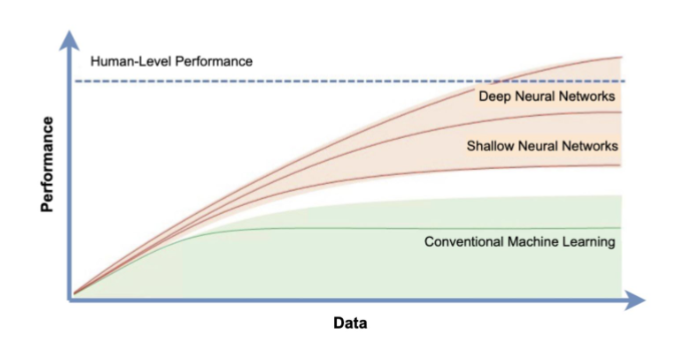
\includegraphics[width=0.75\linewidth]{deeplearning.png}
    \caption{Deep Learning}
    
    \label{fig:enter-label}
\end{figure}
\begin{definition}
"\textbf{Deep learning} is a subset of machine learning that allows \textbf{multiple levels of
representation}, obtained by composing simple but \textbf{non-linear modules} that
each transform the representation at one level \textbf{(starting with the raw input)}
into a representation at a higher, slightly more \textbf{abstract level}." (LeCun et al. 2015)
\end{definition}
\begin{figure}[h!t]
    \centering
    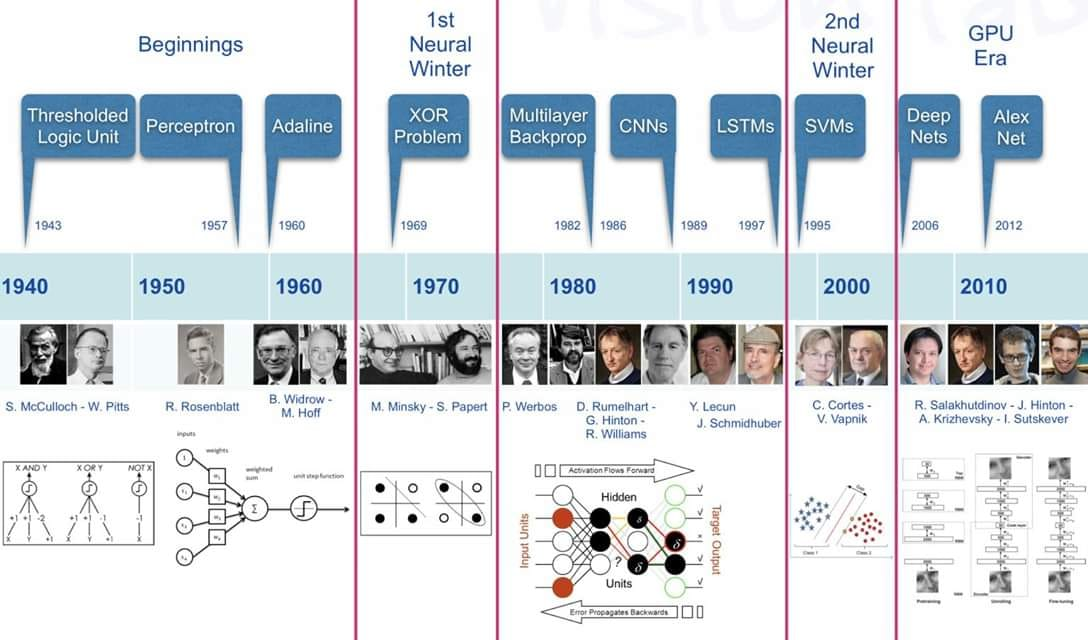
\includegraphics[width=0.75\linewidth]{historydeeplearning.png}
    \caption{History of Deep Learning}
    \label{fig:enter-label}
\end{figure}
\begin{definition}
    \textbf{Artificial Intelligence (AI)}: broad and poorly defined concept of developing computer systems that can \textbf{perform tasks normally only humans could do}. 
\end{definition}
\begin{definition}
    \textbf{Machine Learning (ML)}: computers \textbf{learn by example, from data}, rather than being explicitly programmed, to solve a task. 
\end{definition}
\begin{definition}
    \textbf{Deep Learning (DL)}: a machine learning method that learns \textbf{multiple levels of abstractions} over data end-to-end.
\end{definition}
\begin{figure}[h!t]
    \centering
    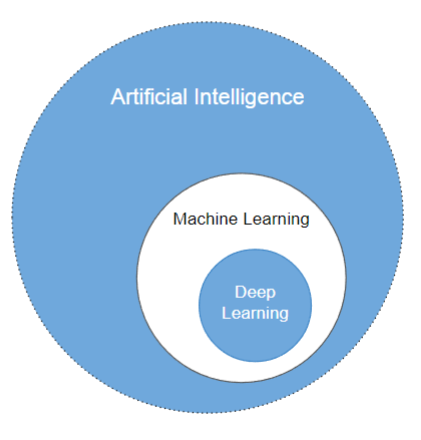
\includegraphics[width=0.25\linewidth]{aimldl.png}
    \caption{Artificial Intelligence vs. Machine Learning vs. Deep Learning}
    \label{fig:enter-label}
\end{figure}
\textbf{\\Deep Learning: Successes}
\begin{itemize}
    \item Machine Translation (Google Translate)
    \item Drug Discovery (antibiotics)
    \item Speech Recognition (auto-generated subtitles)
    \item Image Generation (generate image from prompts)
    \item AlphaFold (protein structures)
    \item AlphaGo
    \item Mathematics (pattern discovery)
    \item Code Generation
    \item Language Modelling
    \item Simulators
\end{itemize}
\textbf{Deep Learning: Caveats}
\begin{itemize}
    \item Interpretability (black box)
    \item Adversarial Examples (noise filters over images)
    \item Causality (while deep learning models excel at identifying patterns in data, they fall short in distinguishing between correlation and causation)
    \item Fairness and Bias
\end{itemize}
\begin{definition}
    \textbf{Bias:} refers to \textbf{systematic and consistent errors or inaccuracies in the predictions or outcomes} produced by a machine learning model. These biases can arise from \textbf{various sources} and can significantly \textbf{impact the model's performance and fairness}. Bias in deep learning can \textbf{occur at different stages} of the model development process, including \textbf{data collection}, \textbf{preprocessing}, \textbf{algorithm design}, and \textbf{decision-making}. 
\end{definition}
\begin{example}
    A 2016 arXiv paper, claimed to be able to predict whether someone was a convicted criminal or not solely from a driver's license-style photo with 90\% accuracy.
When looked at in detail, images of criminals were collected from government IDs, while non-criminal face images were collected from the internet.
\end{example}
    \begin{figure} [h!t]
        \centering
        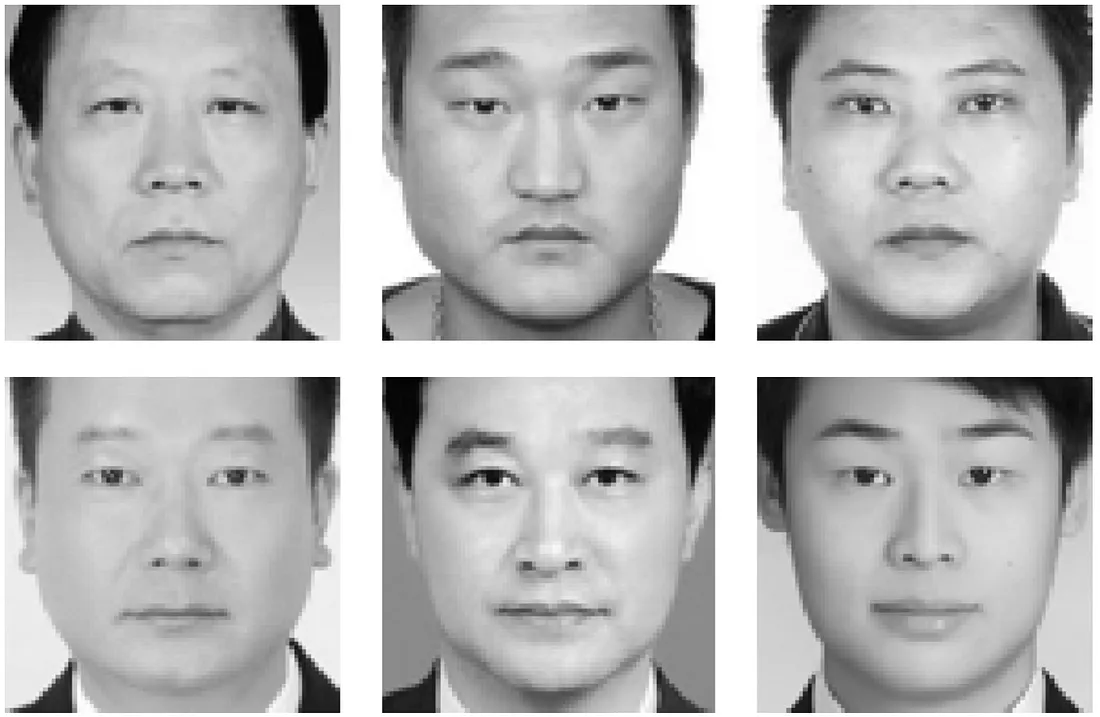
\includegraphics[width=0.5\linewidth]{criminalexamples.png}
        \caption{Top: "criminal" images. Bottom: "non-criminal" images.}
        
    \end{figure}
\section{Machine Learning Basics}

There are three categories that describe how a Neural Network "learns":

\begin{enumerate}
    \item \textbf{Supervised Learning}
\begin{definition}
    \textbf{Supervised Learning:} training by feeding \textbf{labeled data} to the computer, leading it to \textbf{predict the correct label} for inputted data (relationship between input and label)
\end{definition}
\begin{itemize}
\item Involves two main tasks: 
\begin{enumerate}
    \item \textbf{Regression}: the model predicts a continuous or real-valued output
    \item \textbf{Classification}: the model assigns inputs to specific categories or classes
\end{enumerate}
\item Performance is often measured using metrics like \textbf{mean squared error} (for regression) or \textbf{accuracy, precision, and recall (true positive rate) }(for classification)
\item Requires data with \textbf{ground-truth labels}
\end{itemize}
\begin{definition}

            \textbf{Mean Squared Error (MSE):} metric used for measuring the \textbf{average squared difference} between the \textbf{predicted values} and the \textbf{actual (true) values} in a regression problem. It provides a measure of how well a regression model's predictions align with the \textbf{ground truth values}. The lower the MSE value, the better the model's predictions match the data points.\\

\[ \text{MSE} = \frac{1}{n} \sum_{i=1}^{n} (y_i - \hat{y}_i)^2 \]

Where:
\begin{itemize}
\item  \( n \) is the number of data points (samples) in the dataset.
\item \( y_i \) represents the actual target value (ground truth) for the \( i \)th data point.
\item \( \hat{y}_i \) represents the predicted value for the \( i \)th data point by the regression model.
\end{itemize}
\end{definition}

\begin{definition}
    \textbf{Accuracy:} metric that measures the \textbf{proportion of correct predictions} made by a classification model/ It gives an overall view of the model's correctness across all classes.\\
\[ \text{Accuracy} = \frac{\text{Number of Correct Predictions}}{\text{Total Number of Predictions}} \]
\end{definition}

\begin{warning}
Accuracy can be misleading in cases where \textbf{classes are imbalanced}. If one class is significantly more prevalent than others, a model might achieve high accuracy by simply predicting the majority class for all instances.
\end{warning}

\begin{definition}
    \textbf{Precision:} metric that measures the \textbf{proportion of positive predictions} that were actually correct. It measures the model's \textbf{ability to avoid false positives} (instances tat were predicted as positive but are actually negative).\\
\[\text{Precision} = \frac{\text{True Positives}}{\text{True Positives + False Positives}} \] 
\end{definition}

\begin{definition}
    \textbf{Recall (True Positive Rate):} metric that quantifies the \textbf{proportion of actual positive instances} that were correctly predicted by the model. It helps identify the model's ability to \textbf{capture all instances of the positive class}, minimizing false negatives (instances that are actually positive but are predicted as negative). \\
\[ \text{Recall} = \frac{\text{True Positives}}{\text{True Positives + False Negatives}}\]
\end{definition}



\begin{example}
    \textbf{Fitting a polynomial (Regression):} Given a noise sample data (blue), we want to find the polynomial that generated the data.
However, many possible curves fit. Which of these curves is the best fit and why? This is where knowledge of the problem, \textbf{domain knowledge}, can be used to select an appropriate modelling technique.
\end{example}
\begin{figure}[h!t]
    \centering
    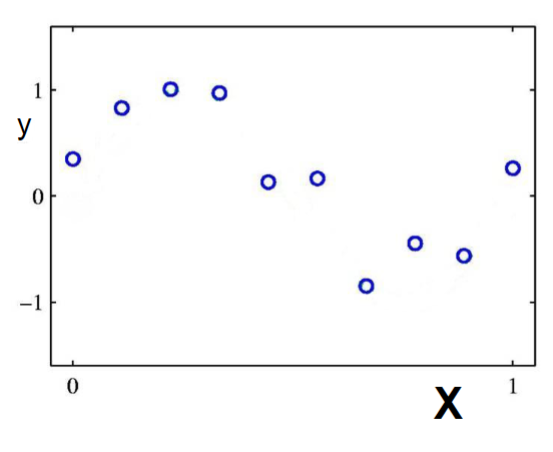
\includegraphics[width=0.5\linewidth]{regressionexample1.png}
    \caption{Noisy Sample Data}
    \label{fig:enter-label}
\end{figure}
\begin{figure}[h!t]
    \centering
    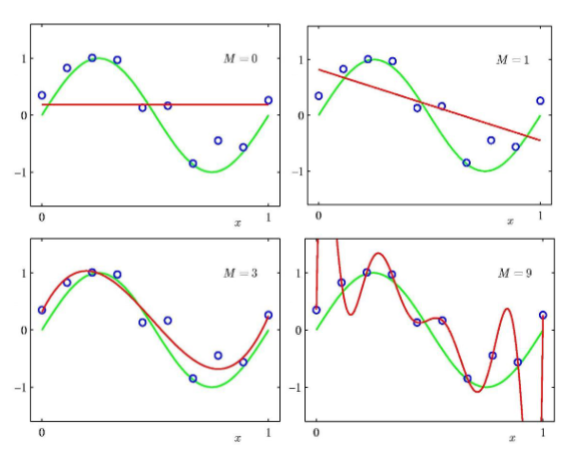
\includegraphics[width=0.5\linewidth]{possiblecurves.png}
    \caption{Possible Curves}
    \label{fig:enter-label}
\end{figure}

\begin{definition}
    \textbf{Inductive Bias (Learning Bias):} set of \textbf{assumptions} used for modelling, or prior knowledge that a learning model \textbf{uses to generalize} from the training data to new, unseen data. It's the foundational principles and constraints that guide a model's learning process and influence the types of patterns it's more likely to learn. Applies to all types of learning.
\end{definition}

\begin{theorem}
\textbf{No Free Lunch Theorem:} concept that \textbf{there is no universal optimization} of learning algorithm that performs best for all possible problems. There is \textbf{no one-size-fits-all approach} that can excel across all domains and problem instances.
\end{theorem}

    \item \textbf{Unsupervised Learning}
\begin{definition}
  \textbf{ Unsupervised Learning:}  training by feeding \textbf{unlabeled data}; hence, relationships are made between \textbf{elements of input} (Clustering, grouping algorithm)
\end{definition}
\begin{itemize}
    \item Requires observations\textbf{ without human annotations}
    \item Also known as Self-supervised Learning or Semi-supervised Learning
\end{itemize}
    \item \textbf{Reinforcement Learning}
\begin{definition}
    \textbf{Reinforcement Learning:} when we want to train a computer to perform a task but \textbf{we don’t know the optimized way} so the computer \textbf{finds the best steps by itself} (we rank the computer’s methods relative to each other and this way the computer learns the best method to perform a task)
\end{definition}
\begin{itemize}
    \item Has an\textbf{ agent}, which is an entity capable of perceiving its environment, making decisions, and taking actions in order to achieve specific goals. This may be a software program, a robot equipped with sensors, or any \textbf{system that interacts with its environment} to acheive desired outcomes. 
    \item \textbf{Sparse rewards} from environment. For example, winning or losing can only occur at the end of a game, making it difficult for an agent to learn to specific actions that lead to victory.
    \item \textbf{Dynamic nature}: agent's actions directly influence the environment. \textbf{Feedback loop} where agent's actions influence the environment, which in turn affects the agent's future options and decisions.

\end{itemize}

\end{enumerate}

\textbf{Machine Learning is a game of balance, with the objective being to generalize training data and future data.}

\begin{definition}
\textbf{Bias:} refers to the \textbf{error introduced by approximating a real-world problem}, which may be complex, with a simplified model. In the context of a machine learning model, bias is the \textbf{error due to overly simplistic assumptions in the learning algorithm}. If a model has high bias, it means that it doesn't capture the underlying patterns in the training data well, leading to systematic errors. In other words, it is "\textbf{underfitting}" the data.
\end{definition}
    
\begin{definition}
\textbf{Variance:} refers to the model's \textbf{sensitivity to small fluctuations or changes} in the training data. A model with high variance tends to fit the training data very closely, even capturing noise or randomness in the data. This can lead to a situation where the model performs well on the training data but poorly on new, unseen data, because it \textbf{hasn't generalized well}. This is called "\textbf{overfitting}."
\end{definition}

\begin{theorem}
    \textbf{Bias-Variance Tradeoff}: as you increase the complexity of a model, you generally reduce bias but increase variance, and vice versa. Finding the right level of complexity that minimizes both bias and variance is crucial for building models that generalize well to new data.

    \begin{itemize}
        \item If you \textbf{increase model complexity} (more features, more layers in neural networks, etc.), the model becomes more flexible and capable of fitting the training data closely. However, it also becomes more sensitive to fluctuations and noise in the data, \textbf{increasing the risk of overfitting} (high variance).
        \item If you\textbf{ decrease model complexity}, the model becomes more constrained and less likely to fit the training data perfectly. While it might generalize better to new data, it could struggle to capture complex patterns, \textbf{resulting in underfitting} (high bias).
    \end{itemize}
\end{theorem}
\begin{idea}
    Generally, \textbf{more data} leads to a better model.
\end{idea}

We need to split our dataset so that it can be use to\textbf{ train, validate, and test }the model. We need to ensure the model does not see the testing (holdout) data during the training process, as that leads to overfitting to the test data and poor generalization on new data. The purpose of validation data is for assessing performance and making informed decisions about model selection and hyper-parameter tuning. 

\begin{figure}[h!t]
    \centering
    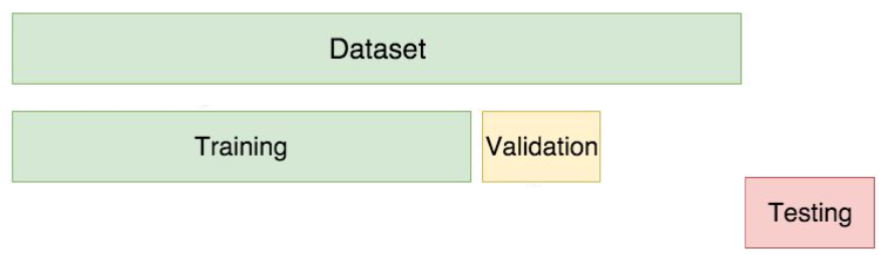
\includegraphics[width=0.75\linewidth]{datatypes.png}
    \caption{Dataset split into Training, Validation, and Testing Datasets}
    \label{fig:enter-label}
\end{figure}

